
\section{Functional Imaging}
\label{sec:functionalimaging}
\begin{onehalfspace}
    
Neuroimaging was developed to investigate the anatomy, activity, and function of the central nervous system, with particular emphasis on the brain. It enables the characterization of when and where neural systems are engaged during sensory, cognitive, or behavioral processes (e.g., memory, language, perception, attention, and emotion regulation) \citep{yenExploringFrontiersNeuroimaging2023}. Neuroimaging modalities differ primarily in the spatiotemporal resolution at which they acquire data (Fig. \ref{fig:imaging}).

Electroencephalography (EEG) and magnetoencephalography (MEG) are electrophysiological neuroimaging techniques that provide high temporal resolution (on the order of $\sim$10–100 ms), at the expense of relatively low spatial resolution (on the order of millimeters to centimeters). These methods enable non-invasive measurement of the electric or magnetic fields generated by ensembles of synchronously active neurons. High spatial resolution recordings of neuronal activity are currently achievable only with invasive approaches, such as patch-clamp recordings, single-unit or multi-unit recordings, and electrocorticography (ECoG).

Functional magnetic resonance imaging (fMRI), positron emission tomography (PET), and magnetic resonance spectroscopy imaging (MRSI) are neuroimaging modalities based on magnetic resonance or nuclear imaging that provide high spatial resolution (on the order of millimeters) for both superficial and deep brain structures, albeit with comparatively low temporal resolution. These methods allow non-invasive assessment of hemodynamic and metabolic processes, such as cerebral blood flow and oxygen utilization, that are associated with neural activity. PET is particularly suitable for quantifying cerebral blood flow (CBF), cerebral blood volume (CBV), and the cerebral metabolic rate of oxygen (CMRO$_2$), whereas fMRI offers superior temporal resolution and is thus more appropriate for detecting changes linked brain responses \citep{heegerSpikesBOLDWhat2000}. MRSI provides information on molecular composition by quantifying the concentrations of ion- or nucleus-specific metabolites within a region of interest. MRSI measurements yield the relative abundance of molecular components in parts per million, based on differences in their resonance frequencies, but this comes at the cost of very low temporal resolution.

Near-infrared spectroscopy (NIRS) and event-related optical signal (EROS) imaging are optical diffusion techniques that quantify cortical hemodynamics using scalp-mounted optical sensors that measure light absorption. These methods are spatially constrained to cortical regions, as photon penetration is limited by scattering and absorption in the skull and overlying tissues. EROS achieves a temporal resolution comparable to that of MEG and EEG, whereas NIRS exhibits temporal characteristics similar to fMRI because it indexes hemodynamic responses \citep{pereiraMultimodalAssessmentSpatial2023, noviRevealingSpatiotemporalRequirements2023}. A key advantage of these optical techniques is that they are relatively low-cost and portable compared to other neuroimaging modalities.

\begin{figure*}
   \centering
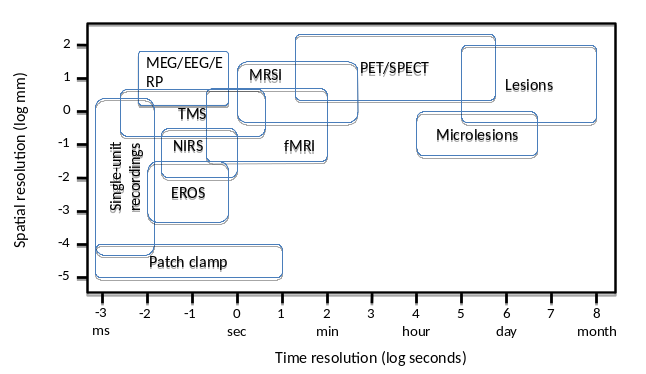
\includegraphics[width=8cm]{images/functional_methods.png}
    \caption[Functional brain imaging techniques]{Spatial and temporal resolutions from different neuroimaging techniques. Figure from \citep{caballerogaudesParadigmFreeMapping2011}}
    \label{fig:imaging}
\end{figure*}

\end{onehalfspace}


\section{fMRI}
\begin{onehalfspace}
    

Magnetic resonance imaging (MRI) enables the detection of functional brain activation by measuring changes in indirect metabolic parameters, such as cerebral blood flow (CBF), cerebral blood volume (CBV), and blood oxygenation. Functional MRI (fMRI) does not require the administration of exogenous contrast agents to assess metabolic changes; instead, it capitalizes on the blood-oxygenation-level-dependent (BOLD) contrast mechanism \citep{ogawaOxygenationsensitiveContrastMagnetic1990, kimPrinciplesBOLDFunctional2023}. This feature, together with its relatively high spatial resolution, has made fMRI a widely used technique in the cognitive neurosciences.

The fMRI signal depends on neurovascular and neurometabolic coupling, that is, the relationship between local neuronal activity and accompanying changes in energy metabolism and hemodynamics during cognitive or sensorimotor events  \citep{uludagIntegrativeModelNeuronal2009a}. Consequently, fMRI is well suited for investigating sensory, motor, and higher-order cognitive processes (e.g., memory, language, and attention) \citep{logothetisWhatWeCan2008, vanderzwaagFMRI1532009, viswanathanNeurometabolicCouplingCerebral2007}. Moreover, fMRI has enabled the identification of large-scale intrinsic brain networks, most notably the default mode network (DMN), which is preferentially active during rest or in the absence of goal-directed attention to external stimuli \citep{menon20YearsDefault2023a}.

Due to their underlying physical properties, fMRI raw data are represented as complex-valued signals (see section \ref{sec:signal}). Consequently, most research has focused predominantly on the magnitude component of the MRI signal for detecting brain activation, typically disregarding the phase component \citep{hagbergPhaseVariationsFMRI2014}. The magnitude corresponds to the absolute value (modulus) of a vector in the complex plane, whereas the phase denotes the angle that this vector forms with respect to the real axis (Figure \ref{fig:complex}).

\end{onehalfspace}

\subsection{Blood Oxigenation Level-Dependent effect (BOLD)}
\label{sec:BOLD}

\begin{onehalfspace}
The blood-oxygen-level-dependent (BOLD) signal arises from differences in oxygenation state of hemoglobin in the blood, which in turn induce alterations in the magnetic properties of the tissue sample \citep{ogawaOxygenationsensitiveContrastMagneticRodent}. Local increases in neuronal activity are accompanied by elevated metabolic demand and, consequently, increased oxygen consumption, which is compensated by an augmented supply of oxygenated blood. When hemoglobin binds molecular oxygen to form oxyhemoglobin, it exhibits diamagnetic behavior (i.e., it weakly repels an external magnetic field), whereas deoxygenated hemoglobin (deoxyhemoglobin) is paramagnetic (i.e., it weakly attracts an external magnetic field) \citep{paulingMagneticPropertiesStructure1936}. 

Deoxyhemoglobin induces more pronounced  magnetic field inhomogeneities than oxyhemoglobin and therefore leads to a faster $T_2^*$ decay, as spin dephasing occurs more rapidly in regions with lower oxygenation. This accelerated dephasing reduces the amplitude of the MR signal. Conversely, when cerebral blood flow and oxygen delivery increase to meet the metabolic demands of neuronal activity, the relative concentration of oxyhemoglobin rises and the local $T_2^*$ decay is reduced, resulting in an increased MR signal. This mechanism underlies functional MRI (fMRI), in which $T_2^*$-weighted images are used to identify brain regions with task- or state-dependent functional activity as inferred from local changes in the balance between oxygen demand and supply. 

\begin{figure*}
   \centering

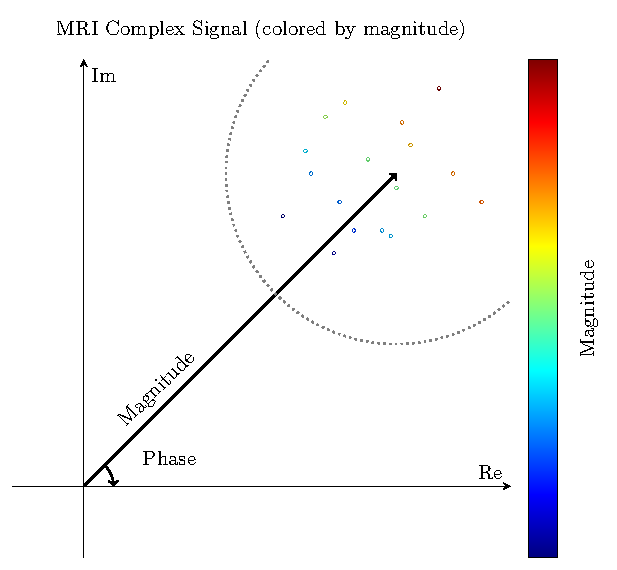
\includegraphics[width=6cm]{images/MRIcomplex.pdf}
    \caption[MRI complex signal]{Magnitude and phase components of the complex MRI signal. The majority of functional MRI (fMRI) studies exclusively analyze the magnitude component to identify task-related or spontaneous brain activations, while the phase information is typically disregarded.}
    \label{fig:complex}
\end{figure*}



Notably, changes in $T_2^*$ because of BOLD effect reflect neural population synaptic behavior and their time dynamics are slower that neuron spiking behaviour \citep{logothetisWhatWeCan2008,viswanathanNeurometabolicCouplingCerebral2007} (see \ref{sec:hrf}). $T_2^*$ values are not uniform across the brain; they vary according to tissue type (e.g., cortical versus subcortical regions) and depend on the orientation of blood vessels and cellular structures relative to the main magnetic field \citep{viessmannDependenceRestingstateFMRI2019, petersT2MeasurementsHuman2007,uludagIntegrativeModelNeuronal2009a}. 

Echo-planar imaging (EPI) sequences are the most frequently employed MRI acquisition schemes for generating $T_2$- or $T_2^*$-weighted images because of their high sensitivity to magnetic field inhomogeneities, such as those induced by the BOLD effect (see \ref{sec:epi}). The effective transverse relaxation rate, $R_2^* = 1/T_2^*$, can be decomposed as
\end{onehalfspace}

\begin{equation}
    R_2^* = R_2 + R_2^{\prime}\text{,}
\end{equation}

\begin{onehalfspace}
where $R_2$ denotes the irreversible (spin–spin) relaxation component and $R_2^{\prime}$ the reversible component arising from microscopic field inhomogeneities.

To minimize $T_1$-weighting and to maximize signal amplitude, the gradient-echo (GE) EPI signal can be modeled as
\end{onehalfspace}

\begin{equation}\label{eq:st}
    S(t) = S_0 e^{-t R_2^*}\text{,}
\end{equation}

\begin{onehalfspace}
where $S_0$ represents the net magnetization, serving as a proxy for the equilibrium magnetization $M_0$. The BOLD-related signal change resulting from a variation in $R_2^*$ is given by
\end{onehalfspace}

\begin{equation}
    \frac{\Delta S}{\Delta R_2^*} = - S_0 t e^{-t R_2^*}\text{.}
\end{equation}

\begin{onehalfspace}
BOLD contrast arises from the interaction between the baseline $T_2^*$ and the echo time. The BOLD contrast is maximized when the echo time $TE$ is approximately equal to $T_2^*$ (see Fig. \ref{fig:boldContrast}). Under this condition, the BOLD contrast can be expressed as
\end{onehalfspace}

\begin{equation}
    \Delta S = -S_0 \cdot \Delta R_2^* \cdot TE \, e^{-TE \cdot R_2^*} 
    = -S \cdot\Delta R_2^* \cdot TE\text{,}
\end{equation}

\begin{onehalfspace}
where the baseline signal is $S = S_0 e^{-TE\, R_2^*}$, and $\Delta R_2^*$ denotes the change in relaxation rate between the activated (BOLD) state and the resting state, i.e., $\Delta R_2^* = R_{2,\text{BOLD}}^* - R_2^*$.

Because $T_2^*$ varies across different brain regions, it is common practice to choose $TE$ shorter than the expected $T_2^*$ in order to reduce inter-voxel susceptibility-induced signal differences, which, however, tends to increase the relative contribution of venous components to the BOLD signal \citep{petersT2MeasurementsHuman2007}. To mitigate this trade-off, $T_2^*$ (or equivalently $R_2^*$) can be estimated by fitting the exponential decay of the $T_2^*$-weighted signal acquired using a multi-echo EPI sequence, in which the signal is sampled at multiple echo times (see \ref{sec:MEfMRI}). This approach compensates for spatial inhomogeneities within the scan and yields improved overall BOLD contrast \citep{posse1999enhancement}.
\end{onehalfspace}


\begin{figure*}
   \centering
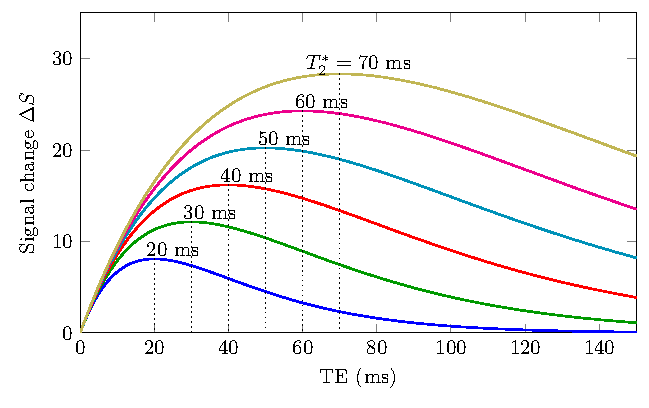
\includegraphics[width=8cm]{images/T2-TE.pdf}
    \caption[BOLD contrast]{Magnitude of the signal change as a function of time for different simulated $T_2^*$ at rest. The maximum BOLD contrast occurs when $TE=T_2^*$}
    \label{fig:boldContrast}
\end{figure*}

\subsubsection{Haemodynamic Response Function (HRF)}
\label{sec:hrf}


\begin{onehalfspace}
Blood-oxygenation-level-dependent (BOLD) functional magnetic resonance imaging (fMRI) constitutes an indirect measure of brain function, as it does not quantify neural activity per se. Instead, fMRI capitalizes on changes in the metabolic demands of neural populations that accompany neuronal processing \citep{finnFunctionalNeuroimagingCatalyst2023,logothetisWhatWeCan2008}. Consequently, the temporal dynamics of the BOLD response are substantially slower than those of the underlying neural activity, because they depend on neurovascular coupling processes.

The hemodynamic response arises from dynamic alterations in cerebral blood flow (CBF), cerebral blood volume (CBV), and the cerebral metabolic rate of oxygen consumption (CMRO$_2$) (see Fig. \ref{fig:hrf}). Immediately following neuronal activation, the local neural population increases its consumption of glucose and oxygen to meet the elevated metabolic demands, which leads to an early decrease in the BOLD signal—often referred to as the initial dip of the hemodynamic response function (HRF) \citep{mullingerPoststimulusUndershootsCerebral2013, chenInvestigatingMechanismsFast2021}. This transient negative deflection is relatively rapid (on the order of $\sim$2 s) and provides spatially precise information regarding the locus of metabolic demand, but it is generally challenging to detect reliably \citep{duongSpatiotemporalDynamicsBOLD2000, mullingerPoststimulusFMRIEEG2017}.

The metabolic stress associated with the initial dip is subsequently counteracted by an increase in local blood flow and blood volume, leading to an influx of oxygenated hemoglobin that overcompensates for the original metabolic demands. This oversupply of oxygenated hemoglobin produces the characteristic positive BOLD response associated with neural activation. Conversely, a negative BOLD response can arise in regions exhibiting neural deactivation or reduced metabolic demand \citep{shmuelNegativeFunctionalMRI2006,shihNewScenarioNegative2009}. This slower component of the HRF typically peaks between approximately 5 and 8 seconds after stimulus onset; however, its precise latency depends on factors such as magnetic field strength, stimulus characteristics, and cortical region \citep{gomezTemporalSpecificityBOLD2024, vanderzwaagFMRI1532009}.

During the return to baseline, an increase in the relative concentration of deoxyhemoglobin is often observed, giving rise to a post-stimulus undershoot that can persist for several seconds before the signal stabilizes. The mechanisms underlying this late negative component remain incompletely understood, and it is still debated whether it is primarily driven by vascular, neural, or metabolic processes \citep{chenOriginsBOLDPoststimulus2009,havlicekEchotimeDependenceBOLD2017}.

In many functional MRI analyses, the hemodynamic response function (HRF) is mathematically approximated by a double-Gamma function, commonly referred to as the canonical HRF \citep{fristonStatisticalParametricMaps1994, gloverDeconvolutionImpulseResponse1999}:
\end{onehalfspace}

\begin{equation}
    h(t)=g(t;a_1,b_1)-\frac{1}{c}g(t;a_2,b_2),
\end{equation}
where $\frac{1}{c}$ is a scaling factor applied to the second Gamma component. Each Gamma component depends on its shape parameter $a$ and scale parameter $b$, and can be expressed as:

\begin{equation}
    g(t;a,b)=\frac{b^a t^{a-1} e^{-bt}}{\Gamma (a)}\text{.}
\end{equation}

The conventional canonical HRF is typically parameterized such that the first Gamma component has a time-to-peak $\frac{a_1}{b_1}$ of 6 s and a dispersion $\frac{a_1}{b_1^2}$ of 1 s, while the second Gamma component has a time-to-peak $\frac{a_2}{b_2}$ of 16 s and a dispersion $\frac{a_2}{b_2^2}$ of 1 s. It is important to note that, although this formulation remains the standard choice for modeling the HRF, empirical evidence indicates that HRFs vary across tissue types and magnetic field strengths.
\begin{figure*}
   \centering
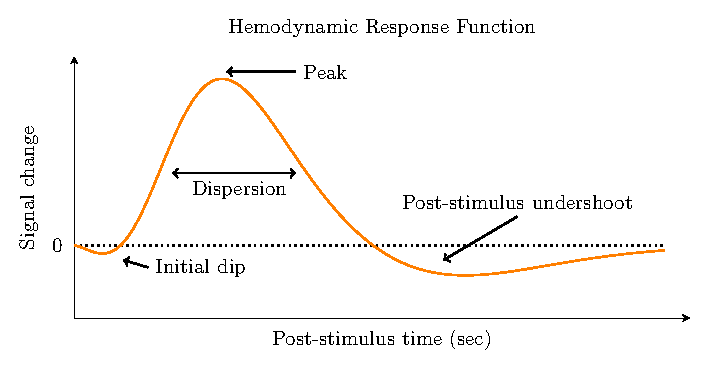
\includegraphics[width=8cm]{images/hrf.pdf}
    \caption[Hemodynamic Response Function (HRF)]{An increase in cerebral blood flow in response to a stimulus is referred to as the hemodynamic response function (HRF). The elevated metabolic demands of neural activity initially induce a transient decrease in oxyhemoglobin concentration, which in turn triggers a compensatory increase in blood flow. Following its peak amplitude, the HRF gradually declines and is typically followed by a post-stimulus undershoot.}
    \label{fig:hrf}
\end{figure*}

\begin{figure}[htbp]
    \centering
    \begin{tabular}{m{7cm}m{5cm}}
    \textbf{(a)} & \textbf{(b)}\\
         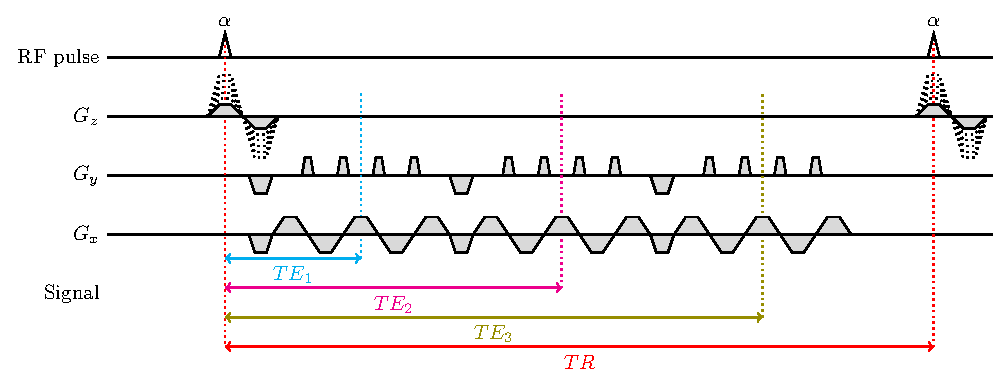
\includegraphics[width=7cm]{images/ME-GE-EPI.pdf} &  
         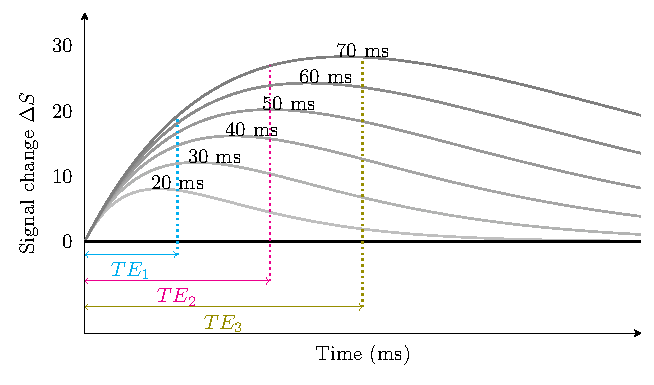
\includegraphics[width=5cm]{images/TET_ME.pdf}\\

    \end{tabular}
    
    \caption[Multi-echo Gradient-echo Echo Planar Imaging sequence]{\textbf{(a)}First TR of a multi-echo gradient-echo echo planar Imaging sequence. After a single RF excitation pulse, $\alpha$, multiple echoes are acquired. \textbf{(b)} Multi-echo acquisition leads to more dense sampling of the all possible $T_2^*$ decay functions, enhancing BOLD sensitivity overall.}
    \label{fig:placeholder}
\end{figure}

\subsection{Multi-echo fMRI}
\label{sec:MEfMRI}

\begin{onehalfspace}
 In single-echo functional magnetic resonance imaging (fMRI), gradient-echo (GE) echo-planar imaging (EPI) acquisition samples the $T_2^*$ decay at an echo time ($TE$) chosen around the relaxation regime of interest in order to maximize blood-oxygen-level-dependent (BOLD) contrast (see Section~\ref{sec:epi}). A key limitation of this single-echo strategy is the spatial heterogeneity of $T_2^*$ across brain tissue, which reduces BOLD contrast and complicates the discrimination between noise and task- or stimulus-related signal changes when interpreting functional effects.

To quantify $T_2^*$ relaxation rates throughout the brain using conventional single-echo approaches, it is necessary to repeat the acquisition at multiple $TE$ values to obtain several sampling points of the underlying relaxation decay curve \citep{posse1999enhancement}. This requirement increases the total experimental duration proportionally to the number of desired $T_2^*$ samples, while largely neglecting the impact of subject motion and other noise sources (see Section~\ref{sec:noiseMRI}).
\end{onehalfspace}



Multi-echo fMRI (ME-fMRI) mitigates these limitations by acquiring multiple echoes following a single radiofrequency (RF) excitation. This strategy enables sampling of the signal decay curve at several echo times within one repetition time (TR), thereby allowing more accurate and robust voxel-wise estimation of $T_2^*$ together with a corresponding time series \citep{heunisEffectsMultiechoFMRI2021}. 
\subsubsection{Multi-echo signal model}
\begin{figure}[htp]
    \centering
    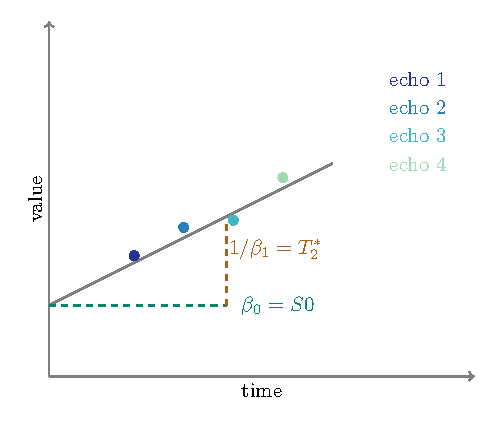
\includegraphics[width=6cm]{images/echo-combination.pdf}
    \caption[S0 and T2 estimation in Multi-echo combination]{S0 and T2 estimation in Multi-echo combination. The parameters $\bar{S_0}$ and $\bar{T_2^*}$ can be expressed as transformations of the model intercept between echoes, $\beta_0$, and slope, $1/\beta_1$, respectively}
    \label{fig:S0T2ME}
\end{figure}
Extending Eq.~\ref{eq:st} to a time-dependent model of $S_0$ and $R_2^*$ yields:
\begin{equation}\label{eq:MEsignal1}
    S(t,TE_k ) = S_0(t,TE_k)\cdot e^{R_2^*(t)\cdot TE_k},
\end{equation}
where $S_0$ and $R_2^*$ can be decomposed into a baseline component and a dynamic component relative to the voxel-wise mean signal: $S_0(t)=\bar{S_0}+\Delta S_0(t)$ and $R_2^*(t)=\bar{R_2^*}+\Delta R_2^*(t)$ \citep{kundu2012differentiating}. Substituting these expressions into Eq.~\ref{eq:MEsignal1} gives:
\begin{equation}\label{eq:MEsignal2}
\begin{aligned}
    S(t,TE_k)
    &= \left(\bar{S_0}+ \Delta S_0(t)\right)\, e^{\left(\bar{R_2^*}+ \Delta R_2^*(t)\right)\cdot TE_k} \\
    &= \bar{S}\left(TE_k\right)\left(1+\frac{\Delta S_0(t)}{\bar{S_0}} \right)\, e^{- \Delta R_2^*(t)\cdot TE_k},
\end{aligned}
\end{equation}
where $\bar{S}\left(TE_k\right)=\bar{S_0}\,e^{-\bar{R_2^*}\cdot TE_k}$. Using the first-order approximation $e^{- \Delta R_2^*(t)\cdot TE_k} \approx 1 - \Delta R_2^*(t)\cdot TE_k$, and defining $\Delta \rho(t) = \frac{\Delta S_0(t)}{\bar{S_0}}$, Eq.~\ref{eq:MEsignal2} can be rewritten as:
\begin{equation}
    S(t,TE_k) \approx \bar{S}(TE_k)\left(1 + \Delta \rho(t) - \Delta R_2^*(t)\cdot TE_k\right).
\end{equation}

Hence, the signal percent change, $y(t,TE_k)=(S(t,TE_k)-\bar{S}(TE_k))/\bar{S}(TE_k)$, relative to the mean signal can then be expressed as:
\begin{equation}\label{eq:spcbold}
\begin{aligned}
    y(t,TE_k) 
    &\approx \Delta \rho(t) - \Delta R_2^*(t)\cdot TE_k. \\
    %&\approx \Delta \rho(t) - TE_k\left(h(t)\cdot \Delta a(t)\right),
\end{aligned}
\end{equation}
%under the assumption that BOLD-induced signal changes in $R_2^*(t)$ can be modeled as $\Delta R_2^*(t) = h(t)\cdot \Delta a(t)$, where $\Delta a(t)$ denotes the latent neural activity–related signal change and $h(t)$ is a canonical hemodynamic response function (HRF; see Sec.~\ref{sec:hrf}).

%If we further assume that the contribution of $\Delta \rho(t)$ is negligible, Eq.~\ref{eq:spcbold} simplifies to a BOLD-only signal percent change model:
%\begin{equation}
%      y(t,TE_k) \approx -TE_k\left(h(t)\cdot \Delta a(t)\right).
%\end{equation}

\subsubsection{Weighted echo combination}

When MRI signals are sampled at multiple echo times (TEs), several strategies are available for combining the resulting echoes, each exploiting distinct advantages. Relative to single‑echo acquisitions, appropriately combined multi‑echo data exhibit increased sensitivity for detecting neural activity, primarily due to the effective reduction of noise achieved during the combination process. To optimize BOLD sensitivity, signals from the different echoes are typically linearly combined using weights that depend on TE and either the voxelwise $T_2^*$ or the temporal signal‑to‑noise ratio (tSNR) as the optimization target \citep{liuGeometricViewSignal2022a}.

 Other approaches perform an unweighted (flat) linear combination of the echoes, or apply weighted summation schemes that explicitly maximize tSNR or contrast‑to‑noise ratio (CNR) \citep{kundu2017multi,liuGeometricViewSignal2022a}. The most commonly adopted strategy is a $T_2^*$‑weighted combination that maximizes CNR by assuming a monoexponential $T_2^*$ decay following a radiofrequency (RF) excitation pulse. This approach is implemented in widely used fMRI preprocessing tools such as tedana (TE‑Dependent ANAlysis) \citep{dupre2021te,kundu2012differentiating}.

Assuming a monoexponential decay model for the MR signal \citep{posse1999enhancement,poser2006bold}, the echo-time–dependent mean signal is modeled as
\[
\bar{S}(TE_k) = \bar{S}_0 \, e^{-\bar{R}_2^* \cdot TE_k},
\]
where \(\bar{S}_0\) denotes the mean signal at \(TE = 0\) and \(\bar{R}_2^*\) is the apparent transverse relaxation rate. Voxel-wise estimates of \(\bar{S}_0\) and \(\bar{R}_2^*\) are typically obtained by applying a log-linear regression to the average signal across the entire time series as a function of echo time. Taking the natural logarithm of the model yields
\[
\log\big(\bar{S}(TE_k)\big) = \log(\bar{S}_0) - \bar{R}_2^* \, TE_k,
\]
which can be expressed in matrix form as
\begin{equation}
    \begin{bmatrix}
        \log\big(\bar{S}(TE_1)\big) \\
        \log\big(\bar{S}(TE_2)\big) \\
        \vdots \\
        \log\big(\bar{S}(TE_k)\big)
    \end{bmatrix}
    =
    \begin{bmatrix}
        1 & -TE_1 \\
        1 & -TE_2 \\
        \vdots & \vdots \\
        1 & -TE_k
    \end{bmatrix}
    \begin{bmatrix}
        \log(\bar{S}_0) \\
        \bar{R}_2^*
    \end{bmatrix}.
\end{equation}
The parameter vector \(\big[\log(\bar{S}_0),\, \bar{R}_2^*\big]^\top\) can then be estimated via the Moore–Penrose pseudoinverse of the design matrix:
\begin{equation}
    \begin{bmatrix}
        \log(\bar{S}_0) \\
        \bar{R}_2^*
    \end{bmatrix}
    =
    \mathrm{pinv}
    \begin{pmatrix}
        \begin{bmatrix}
            1 & -TE_1 \\
            1 & -TE_2 \\
            \vdots & \vdots \\
            1 & -TE_k
        \end{bmatrix}
    \end{pmatrix}
    \begin{bmatrix}
        \log\big(\bar{S}(TE_1)\big) \\
        \log\big(\bar{S}(TE_2)\big) \\
        \vdots \\
        \log\big(\bar{S}(TE_k)\big)
    \end{bmatrix},
\end{equation}
where \(\mathrm{pinv}(\cdot)\) denotes the  pseudoinverse  and \(\log(\cdot)\) is the natural logarithm. After fitting this linear regression model to the vector
\[
    \begin{bmatrix}
        \log(\bar{S}_0) \\
        \bar{R}_2^*
    \end{bmatrix},
\]
the parameters $\bar{S_0}$ and $\bar{T_2^*}$ can be expressed as transformations of the model intercept, $\beta_0$, and slope, $1/\beta_1$, respectively (see Fig ~\ref{fig:S0T2ME}): 
\begin{equation}
\begin{aligned}
    &S_0 = e^{\beta_0} \\
    &T_2^* = \frac{1}{R_2^*} = \frac{1}{\beta_1}\text{.}
    \end{aligned}
\end{equation}



\begin{figure}[htbp]
    \centering
    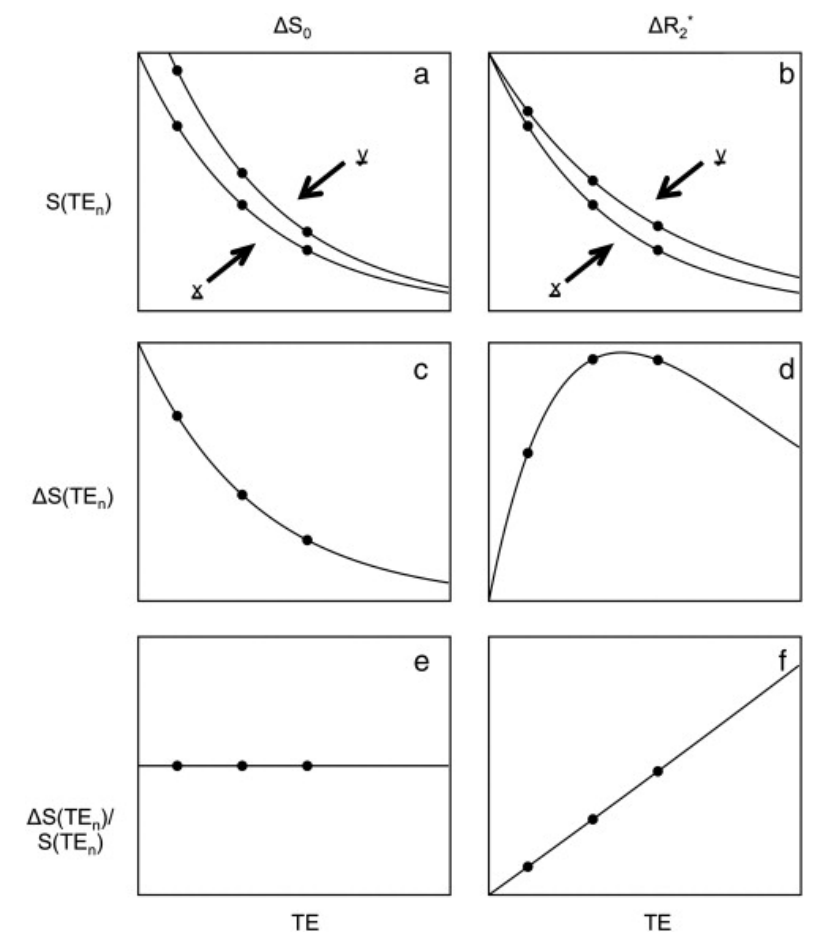
\includegraphics[width=6cm]{images/ME-R2S0.png}
    \caption[BOLD and non-BOLD differentiation with multi-echo fMRI]{TE-independence of non-BOLD versus TE-dependence of BOLD fMRI signal changes between baseline $x$ and activity $y$. a) Exponential decay of $S_0$ through TEs. b) Exponential decay of $\Delta R_2^*$ through TEs. c) Temporal dynamics of $\Delta S$ when attributed to change in $S_0$. d) Temporal dynamics of $\Delta S$ when attributed to changes in $\Delta R_2^*$}
    \label{fig:ME_S0R2}
\end{figure}

\begin{onehalfspace}
Once the transverse relaxation constant is estimated, signal from the multiple echoes can be combined, optimal combination \citep{kundu2012differentiating}, with a weighted sum. Weights depends on the $T_2^*$ decay function as stated in:

\begin{equation}
    w_n^{T_2^*}=\frac{TE_n \cdot e(-TE_n/T_2^*)}{\sum_{i=1}^NTE_i\cdot e(-TE_i/T_2^*)} \text{.}
\end{equation}


Optimal combination of the fMRI signal across multiple echoes enhances overall signal quality by exploiting the distinct contrast and signal amplitude characteristics associated with each echo time. Early echo times ($TE$s) yield high signal intensity but exhibit limited contrast between gray matter, white matter, and cerebrospinal fluid (CSF). Intermediate $TE$s are characterized by reduced signal intensity but improved tissue contrast. Late $TE$s provide the lowest signal intensity while maximizing contrast arising from slowly decaying tissue components \citep{kundu2017multi,heunisEffectsMultiechoFMRI2021}.

\subsubsection{TE-dependent denoising} 


Multi-echo acquisitions facilitate the separation of BOLD and non‑BOLD signal components (e.g., via multi-echo independent component analysis, ME‑ICA) by exploiting their differential fit to either $S_0$‑based ($T_1$‑relaxation–dominated) or $R_2^*$‑based ($T_2$‑relaxation–dominated) models. This biophysical contrast enhances statistical effect sizes and remains one of the most widely used approaches for denoising in multi‑echo fMRI studies \citep{kundu2012differentiating, dupre2021te, kunduIntegratedStrategyImproving2013a, poser2006bold, poserInvestigatingBenefitsMultiecho2009}.

In ME-ICA, goodness-of-fit statistics are then computed on a voxel-wise basis using an F-test that compares the residuals from a candidate model to those from a null model. For each model, the F-statistic is calculated with 1 degree of freedom (DOF) for the model parameter and $n-1$ DOF for the residuals, where $n$ is the number of echoes. The resulting time-series F-values can be averaged across time points, weighted by signal power:
\begin{equation}\label{eq:F}
    \alpha _v=\sum _i ^n \Delta S_{TE_{i}}^2\text{,}
\end{equation}

which yields two summary metrics:
\begin{equation}
    \kappa=\frac{\sum _v ^m \alpha _vF_{v,\Delta R_2^*}}{\sum _v ^m \alpha _v}\text{,}
\end{equation}
and
\begin{equation}
    \rho=\frac{\sum _v ^m \alpha _vF_{v,\Delta S_0}}{\sum _v ^m \alpha _v}\text{.}
\end{equation}

$\kappa$ and $\rho$ are subsequently employed to rank the degree to which a component conforms to signal variations as characterized by $\Delta S_0$ or by $\Delta R_2^*$. The F-values are weighted such that both ranking metrics become less sensitive to ICA estimation errors in components exhibiting small signal changes. 

Although this strategy has been shown to enhance BOLD sensitivity, Eq. \ref{eq:spcmatrix} reveals that the underlying approximation presumes that signal is predominantly driven by positive, time-dependent variations in $\Delta R_2$. This assumption holds provided that no additional time-dependent sources of measurement error or noise are present. For example, subject motion within the scanner, when temporally correlated with the task, such as during speech production, can yield a component that aligns more closely with $\kappa$ than with $\rho$, while still representing a non-BOLD source of signal variation.
\end{onehalfspace}
%explicr secuenci multiecho T2, S0 etc OC over magnitude

\section{Noise sources in fMRI}
\sectionmark{Noise sources in fMRI}
\label{sec:noiseMRI}
\begin{onehalfspace}
The fMRI signal does not arise exclusively from neural activity. Instead, it also contains noise components whose magnitude can be comparable to that of neural activity–related fluctuations, thereby limiting sensitivity to functional activation\citep{liu2016noise, jorgeSignalFluctuationsFMRI2013, bianciardiSourcesFunctionalMagnetic2009}.

The total variance in the fMRI time series can be expressed as the sum of multiple noise sources (see Fig.~\ref{fig:noiseSources}):
\begin{equation}\label{eq:sigma}
    \sigma^2=\underbrace{\sigma _T^2+\sigma _S^2}_\text{$\sigma _0^2$ }+\underbrace{\sigma _B^2+\sigma _{NB}^2}_\text{$\sigma _P^2$ }\text{,}
\end{equation}


where $\sigma_0^2$ represents signal fluctuations independent of the underlying MR contrast, such as thermal noise originating from the subject and electronics ($\sigma_T^2$), and hardware-related noise ($\sigma_S^2$). The term $\sigma_P^2$ comprises physiological signal sources that are dependent on the MR signal (see Sec.~\ref{sub:physio}). Within this category, $\sigma_B^2$ includes BOLD-related fluctuations, such as those driven by changes in cerebral metabolic rate of oxygen consumption ($CMRO_2$), cerebral blood volume ($CBV$), and cerebral blood flow ($CBF$), whereas $\sigma_{NB}^2$ denotes non–BOLD-related physiological contributions, including cardiac pulsation, respiration, and subject motion (see Secs.~\ref{sub:motion}, and~\ref{sub:thermal}). 

$\sigma_P$ fluctuations are proportional to $\Delta S$ when they are BOLD related and can be expressed in interaction with a constant $c_1$ such that $\sigma_B =c_1\Delta S$, whereas non-BOLD physiological fluctuations are expressed as an interaction between signal and a constant $c_2$ such that $\sigma_{NB} = c_2S$ \citep{krugerNeuroimaging15302001}. Then physiological noise is stated as $\sigma_P=\lambda S$, where:
\begin{equation}\label{eq:phys}
    \lambda^2=c_1^2(\Delta R_2^*)^2\ TE^2+c_2^2
\end{equation}


A standard quantitative metric to characterize acquisition performance in terms of the balance between signal of interest and noise is the temporal signal-to-noise ratio ($tSNR$):
\begin{equation}
    tSNR=\frac{\overline{S}}{\sqrt{\sigma^{2}_{0}+\sigma^{2}_{P}}}\text{,}
\end{equation}
where $\overline{S}$ denotes the temporal mean of the signal amplitude. By substituting Eqs.~\ref{eq:sigma} and \ref{eq:phys}, $tSNR$ can be rewritten as

\begin{equation}
    tSNR = \frac{SNR_0}{\sqrt{1 + \lambda^2 SNR_0^2}}\text{,}
\end{equation}
where $SNR_0 = S/\sigma_0$ denotes the signal-to-thermal-noise ratio. As $SNR_0$ increases, $tSNR$ approaches an asymptotic limit of $1/\lambda$ (see Fig.~\ref{fig:tsnr/snr}). If we further assume that $SNR_0$ arises from the dependence on the acquisition voxel volume $v$ with proportionality constant $\kappa$, then the relationship between $tSNR$ and $v$ can be expressed as

\begin{equation}\label{eq:tsnrvolume}
    tSNR = \frac{\kappa \cdot v}{\sqrt{1 + \lambda^2 \cdot \kappa \cdot v}}\text{.}
\end{equation}


From Eq.~\ref{eq:tsnrvolume}, it follows that thermal noise contributes more strongly to the overall variance at high spatial resolution (small voxel volumes) and at fast acquisitions, whereas physiological noise components become increasingly dominant as voxel size is increased or acquisition speed is reduced.

In principle, reducing the variance associated with signals of no interest enhances sensitivity to detect functionally relevant changes, since a decrease in the denominator leads to an increase in $tSNR$. However, attempts to reduce $\sigma^2$ carry the risk of inadvertently attenuating variance attributable to the signal of interest or introducing bias into the data, potentially resulting in spurious effects \citep{kay2022risk}.
\begin{figure}[htbp]
    \centering
    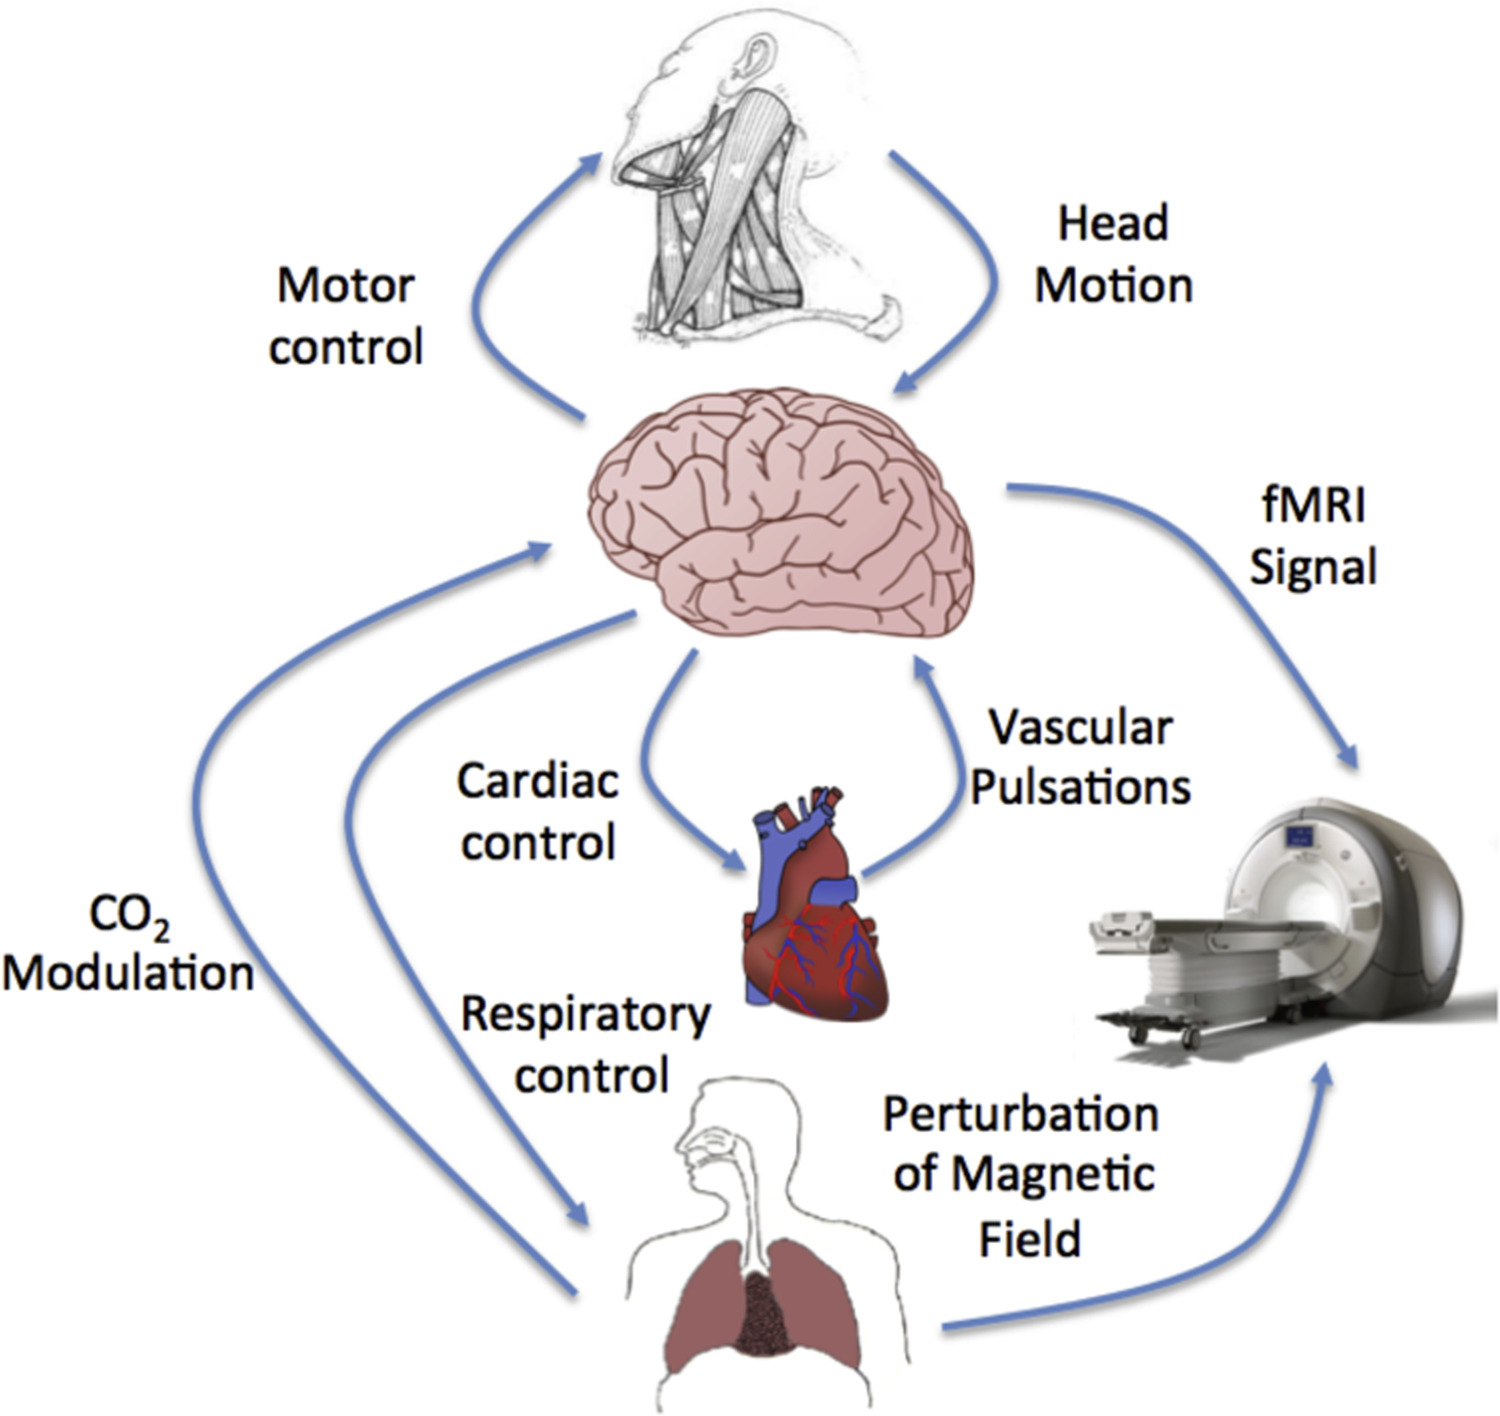
\includegraphics[width=6cm]{images/noise_sources.jpg}
    \caption[Noise sources in fMRI acquisitions]{Schematic representation of the principal noise sources that degrade BOLD (blood-oxygen-level-dependent) contrast in functional MRI. Physiological noise sources include cardiac and respiratory fluctuations; motion-related noise arises predominantly from head movement; and thermal noise originates from electronic components and MRI hardware. Image adapted from \citep{liu2016noise}.}
    \label{fig:noiseSources}
\end{figure}
\begin{figure}[htbp]
    \centering
    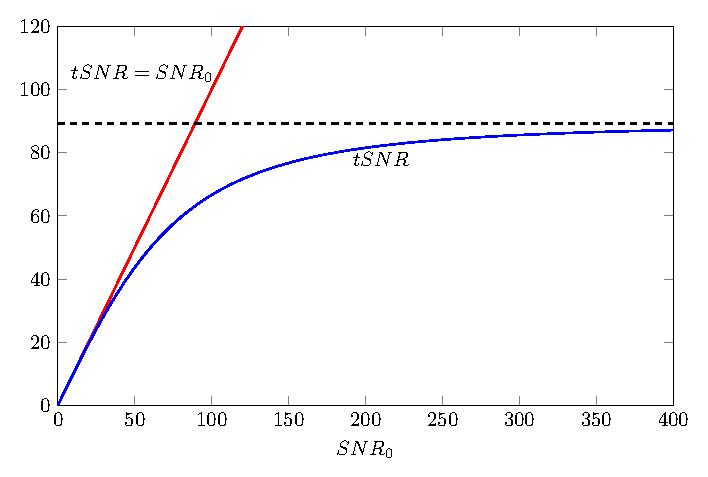
\includegraphics[width=8cm]{images/tsnr-snr0.pdf}
    \caption[Relationship between $tSNR$ and $SNR_0$]{Relationship between $tSNR$ and $SNR_0$. The red line represents an idealized scenario characterized by a linear increase such that $tSNR = SNR_0$. The blue line illustrates that, as $SNR_0$ increases, $tSNR$ approaches an asymptotic limit. Because thermal noise contributes more substantially at high spatial resolutions, one strategy to mitigate regimes with high $SNR_0$ is to increase the voxel size.}
    \label{fig:tsnr/snr}
\end{figure}
\end{onehalfspace}



%relqacion voxel swize, tipos de noise, phisiological noise
\subsection{Physiological Noise}
\label{sub:physio}

\begin{onehalfspace}
 BOLD contrast relies on hemodynamic alterations to indirectly infer neural population activity, it is also susceptible to capturing nuisance signals arising from changes in the neurovascular system that do not have a genuine neuronal origin. More specifically, the oxygen sensitivity of MRI measurements renders respiratory and cardiac cycles major physiological confounds in the MRI signal \citep{caballero2017methods, moia2021ica, kruger2001physiological, addehPhysiologicalConfoundsBOLDfMRI2025}. The influence of these confounding signals is particularly pronounced in the vicinity of large blood vessels, thereby degrading BOLD sensitivity as vascular structures increase in size and depending on their orientation relative to $S_0$ \citep{menonPostacquisitionSuppressionLargevessel2002,vuUsingNovelSourcelocalized2015, uludagIntegrativeModelNeuronal2009a, viessmannDependenceRestingstateFMRI2019}.

Cardiac cycles exert a pulsatile effect on cerebral blood flow (CBF) and cerebral blood volume (CBV). This induces periodic changes in the local concentration of oxygenated blood within a region of interest and, additionally, elicits small tissue displacements synchronized with heart rate. Cardiac-related fluctuations are faster than the canonical BOLD response and typically exhibit a frequency of approximately $1 \,\text{Hz}$.

Respiration modulates arterial $CO_2$ concentration, which exerts a vasodilatory effect on cerebral vessels, thereby increasing CBF and CBV. Variations in respiratory rate and depth directly affect BOLD contrast sensitivity. Furthermore, breathing induces natural head motion and contributes to magnetic field inhomogeneities through changes in chest and airway gas content. Respiratory fluctuations are generally faster than the BOLD signal and are typically observed at a frequency of approximately $0.3 \,\text{Hz}$.

Assuming these physiological sources constitute non-neuronal confounds of the BOLD contrast, several procedures can be applied to attenuate their impact, such as high-pass filtering or regressing out their signal components using ICA or RETROICOR. However, all such approaches carry an inherent risk of attenuating or removing part of the neural signal of interest \citep{caballero2017methods, addehPhysiologicalConfoundsBOLDfMRI2025}.

\end{onehalfspace}

\subsection{Motion-induced noise}
\label{sub:motion}
\begin{onehalfspace}
    

MRI acquisition and BOLD contrast are predicated on the assumption that tissue remains spatially stationary over time. In practice, this assumption is violated. During fMRI acquisitions, participants inevitably move within the scanner, which introduces systematic confounds into the MR signal and degrades both the BOLD contrast and its sensitivity \citep{satterthwaite2019motion,fristonMovementRelatedEffectsFMRI1996}. 

The primary (first-order) effect of motion is voxel displacement during the acquisition of the time series. When a participant moves by as little as one voxel in any direction, the time series associated with that voxel may represent signals originating from different tissue locations across time, thereby blurring the spatial specificity of MRI (see Sec.~\ref{sec:functionalimaging}). This problem is particularly relevant for source localization because, over the course of a typical scan, participants may exhibit multiple translations along the $x,y,z$ axes as well as rotations. Such movements can produce displacements both within tissue classes (e.g., one gray-matter patch replacing another within a voxel) and between different tissue types (e.g., gray matter being replaced by cerebrospinal fluid, white matter, or vascular structures).

The secondary (second-order) effects of motion arise from deviations from the assumed magnetization evolution, in which gradients and RF pulses no longer satisfy the linearity assumptions underlying image reconstruction (see Sec.~\ref{sec:epi}). In the absence of displacement, spins within a brain region are excited at regular intervals, leading to approximately constant saturation and recovery dynamics. Under motion, however, spins experience inconsistent saturation and recovery, and their interaction with the magnetic fields no longer conforms to the expected model. This mismatch can shift the apparent spatial position of spins and thereby introduce reconstruction artifacts and geometric distortions.

The impact of motion on fMRI studies also depends on the experimental paradigm, differing between task-based and resting-state acquisitions. In resting-state fMRI, motion is particularly problematic because it can strongly bias functional connectivity estimates (e.g., voxelwise or region-of-interest-wise time-series correlations). Motion-related artifacts can be mitigated using methods such as rigid-body realignment, motion censoring, scrubbing, and distortion correction based on field maps \citep{caballero2017methods,liu2016noise}.


\end{onehalfspace}

\subsection{Thermal noise}
\label{sub:thermal}
\begin{onehalfspace}
BOLD contrast is constrained by spatially independent variance components arising from hardware and electronic sources, collectively referred to as thermal noise. Thermal noise originates from thermally induced, stochastic current fluctuations that perturb the magnetic field within the sample, and its influence is particularly prominent in low–signal-to-noise ratio (SNR) regimes\citep{bodurkaMappingMRIVoxel2007,edelsteinIntrinsicSignaltonoiseRatio1986,houltSignaltonoiseRatioNuclear2011}.

Thermal noise is statistically independent across measurements and is temporally and spatially uncorrelated with the MRI timeseries of interest. Prior to data reconstruction via the Fourier transform in the complex domain, where the real and imaginary components are mutually orthogonal (see Sec.~\ref{subsec:kspace} and Fig.~\ref{fig:complex}), thermal noise is well described by a zero-mean Gaussian distribution. Following reconstruction into magnitude and phase images, the effective noise distribution in the magnitude data deviates from Gaussianity and instead follows a Rician distribution  (see Fig.~\ref{fig:ricean}), whereas noise distribution in the phase data remains cero centered \citep{gudbjartssonRicianDistributionNoisy1995c} . 

Currently the tendency within fMRI research is to move towards high resolution spatial sampling (i.e., smaller voxel size) and/or high resolution temporal sampling acquisitions (i.e., faster TRs, faster echoe time(s), parallel image reconstruction). Higher magnetic field scanners, Multi-channel/array coil configurations alongside high-accelerated acquisition like the ones popularized by the human connectome project have made possible these despite of increasing the g-factor. The trade-off is pushing MRI signal to a lower SNR regime, where thermal noise dominates over physiological noise  \citep{triantafyllouComparisonPhysiologicalNoise2005,triantafyllouPhysiologicalNoiseSignaltonoise2011,bodurkaMappingMRIVoxel2007}.


\begin{figure}[htbp]
    \centering
    \begin{tabular}{m{3cm}m{3cm}}
      \textbf{(a)}   & \textbf{(b)} \\
        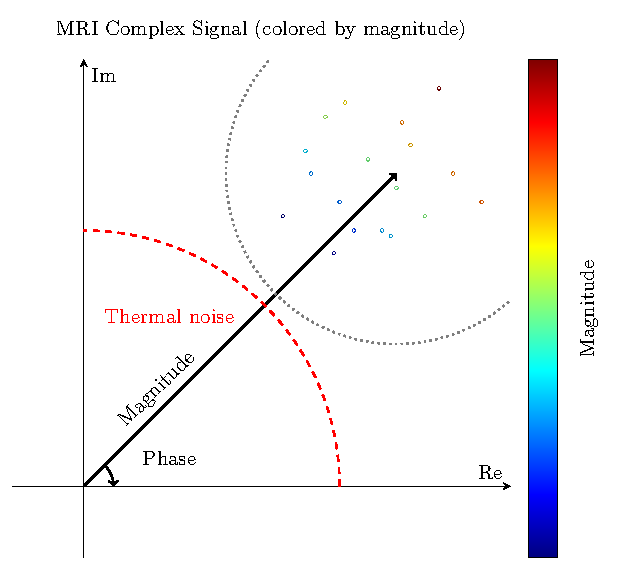
\includegraphics[width=3cm]{images/MRIthermal.pdf} & 
        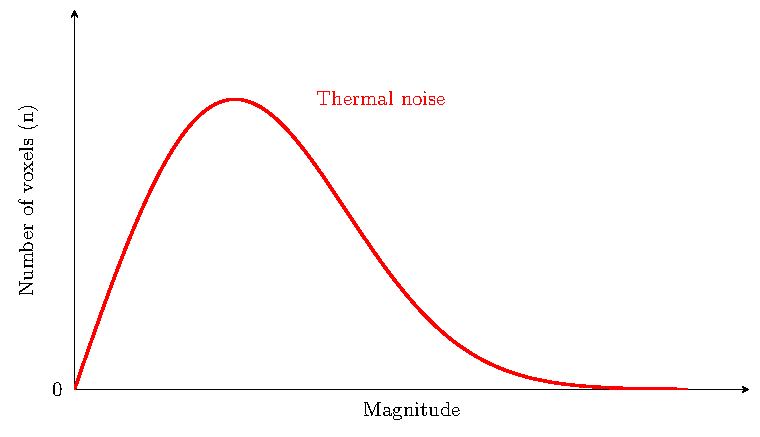
\includegraphics[width=3cm]{images/ricean.pdf}
    \end{tabular}
    \caption[Thermal noise as a Rician distribution]{Transformation of thermal noise characteristics when moving from the complex to the magnitude domain. \textbf{(a)} In the complex domain, thermal noise is approximately Gaussian, isotropic, and centered at zero. \textbf{(b)} In the magnitude-only representation of the MRI signal, thermal noise is neither uniform nor centered at zero; instead, it follows a Rician distribution, with a characteristic positive bias that extends into higher magnitude values.}
    \label{fig:ricean}
\end{figure}
    

    
\end{onehalfspace}

\subsection{Reducing thermal noise in fMRI}
\begin{onehalfspace}
    

Given the inherently unstructured and skewed nature of thermal noise, most denoising strategies do not explicitly target this source of variance (e.g., via band‑pass filtering). Instead, spatial smoothing, multi‑echo (ME) denoising, and low‑rank approaches are among the most commonly employed techniques to mitigate thermal noise \citep{comby2023denoising, talagalaCorrectionSignalDrift1999, triantafyllouEffectSpatialSmoothing2006}. However, the majority of these methods have been primarily designed for single‑echo acquisitions and/or do not fully exploit the specific advantages afforded by ME $T_2^*$‑weighting; systematic application of such approaches remains to be thoroughly investigated.

Spatial smoothing denotes a procedure that increases the signal‑to‑noise ratio (SNR) at the cost of reduced spatial resolution. In spatial smoothing, the time series of each voxel is replaced by a weighted average of the time series from spatially neighboring voxels defined by a convolution kernel. This smoothing kernel is most commonly Gaussian, characterized by a full width at half maximum (FWHM) typically on the order of 5, 8, or 12 mm. By averaging nearby voxel time series, spatially incoherent noise is attenuated and large‑scale trends in the signal become more prominent at the expense of spatial precision. This spatial blurring is particularly undesirable in high‑resolution acquisitions, as it effectively negates their inherent advantage. Furthermore, spatial smoothing has been shown to alter voxel‑wise and region‑to‑region functional connectivity estimates, potentially leading to biased or misleading conclusions \citep{alakorkkoEffectsSpatialSmoothing2017, triantafyllouEffectSpatialSmoothing2006}.

Beyond enabling voxel‑wise, optimally weighted combination of multiple echoes, multi‑echo fMRI (ME‑fMRI) offers specific benefits for thermal noise attenuation (see Fig. \ref{fig:ME_S0R2}). Individual echoes differ in their $T_2^*$‑weighting and thermal noise properties while exhibiting essentially identical $T_1$‑weighting. Acquiring a sufficiently short echo time (TE) yields a minimally $T_2^*$‑weighted signal that can be used, in conjunction with later, more BOLD‑sensitive echoes, to model and regress out fluctuations in $S_0$, which are assumed to be predominantly driven by thermal noise \citep{caballero2017methods, talagalaCorrectionSignalDrift1999, brightRemovingMotionPhysiological2013}. A key limitation of this strategy is that both hardware and software constraints restrict how early the first echo can be sampled at high spatial resolutions, as well as how many subsequent echoes can be acquired. Moreover, pushing the scanner towards faster acquisitions generally reduces the SNR, thereby increasing the relative contribution of thermal noise.

Low‑rank denoising encompasses a class of techniques that rely on the assumption that nuisance variability can be isolated and attenuated by exploiting redundancy in the data matrix via principal component analysis (PCA) \citep{zhu2022denoise,marcenkoDistributionEigenvaluesSets1967a}. These approaches typically assume that the structured signal of interest, and thus the majority of the variance, is captured by a limited number of high‑variance components, whereas noise is distributed across many components and is predominantly represented in those with the lowest variance. These methods will be discussed in greater detail in the following subsection.
\end{onehalfspace}

\subsection{Low-rank denoising methods}

\begin{onehalfspace}

\subsubsection{MPPCA}
\begin{figure}[htbp]
    \begin{tabular}{m{7cm}m{3cm}}
        \textbf{(a)} & \textbf{(b)}  \\
        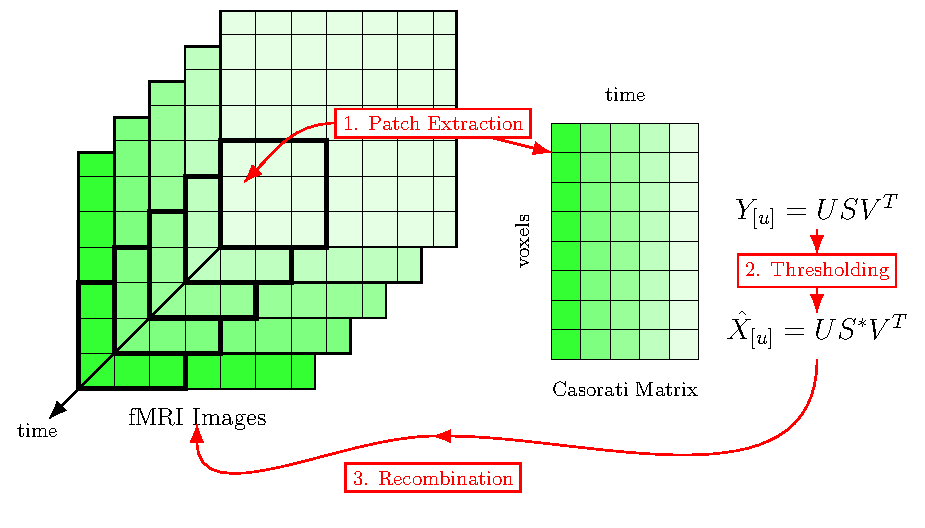
\includegraphics[width=7cm]{images/MPthreshold.pdf}  & 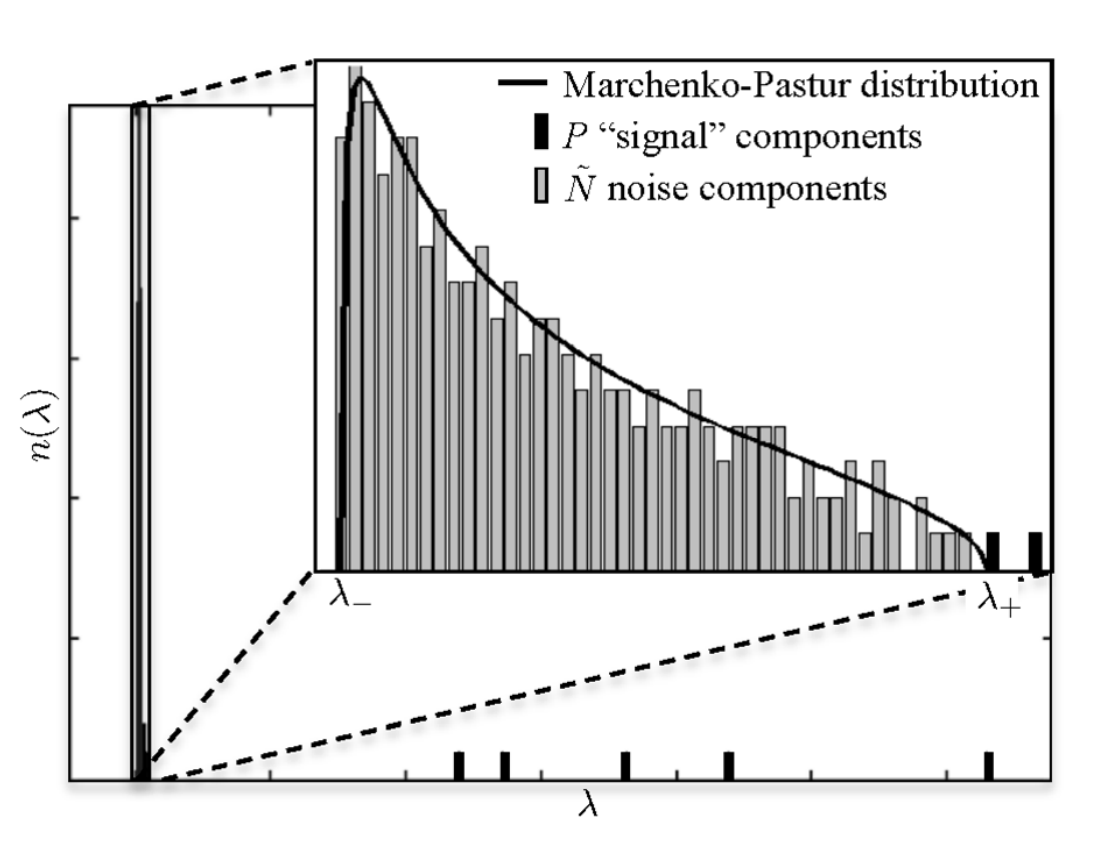
\includegraphics[width=3cm]{images/MPdistribution.png}
    \end{tabular}
    
    \caption[Low-rank methods for denoising]{\textbf{(a)} Illustration of low-rank denoising for a two-dimensional dataset for visualization purposes. A local patch is extracted and reshaped into a Casorati matrix, which is then decomposed into its eigenvalues (or singular values) $\lambda$ and ordered according to the Marchenko–Pastur distribution shown in \textbf{(b)}. Eigenvalues identified as noise-dominated are thresholded, and the corresponding matrix is subsequently recomposed to obtain a denoised fMRI time series. Images adapted from \citep{comby2023denoising,veraartDiffusionMRINoise2016}}
    \label{fig:mp}
\end{figure}
Low-rank denoising methods exploit the inherent redundancy of information in MRI acquisitions to identify and suppress noise variance. These methods rely on the Marchenko–Pastur law from random matrix theory (RMT), which characterizes the eigenvalue distribution of noisy covariance matrices and states that eigenvalues dominated by noise account for a comparatively small proportion of the total variance of the original matrix \citep{marcenkoDistributionEigenvaluesSets1967a,veraart2016denoising}. Functional MRI (fMRI) data are intrinsically low-rank because the BOLD contrast arises from small signal fluctuations over time superimposed on a relatively large and slowly varying background (see Sec. \ref{sec:signal}); consequently, the temporal fMRI signal exhibits strong correlations across time points.

Consider a local patch of an fMRI acquisition centered on voxel $u$, denoted by $\mathbf{Y}_{[u]}$. This patch can be represented as a redundant Casorati matrix of dimensions $M \times N$, with $R \equiv \min\{M, N\} \geqslant 1$. Here, $M$ corresponds to the number of voxels in the patch (spatial dimension), and $N$ to the number of time points (temporal dimension). The matrix $\mathbf{Y}_{[u]}$ is modeled as a noisy observation of a low-rank matrix,
\[
\mathbf{Y}_{[u]} = \mathbf{X}_{[u]} + \mathbf{N}(\sigma^2_{[u]}),
\]
where $\mathbf{X}_{[u]}$ is the underlying noise-free signal, and $\mathbf{N}$ is a zero-mean Gaussian noise matrix with variance $\sigma^2_{[u]}$. The matrix $\mathbf{Y}_{[u]}$ can be approximated as a linear combination of a small number of linearly independent sources, or principal components, with $P \geqslant R$ (see Fig.~\ref{fig:mp}). For convenience, $\mathbf{Y}_{[u]}$ can be regarded as a high-dimensional measurement that is effectively constrained to a $P$-dimensional subspace:

\begin{equation}\label{eq:svd}
    \mathbf{Y}_{[u]} = \mathbf{U}\mathbf{S}\mathbf{V}^T,
\end{equation}
where $\mathbf{U}$ is an $M \times M$ complex unitary matrix, $\mathbf{S}$ is an $M \times N$ diagonal (or rectangular diagonal) matrix containing the singular values $\lambda_1, \ldots, \lambda_R$ on its main diagonal, and $\mathbf{V}$ is an $N \times N$ complex unitary matrix.

Low-rank methods focus on the distribution of the singular values (or, equivalently, eigenvalues of the covariance matrix), which are sorted such that $\lambda_1 \geq \lambda_2 \geq \cdots \geq \lambda_R$. Because the covariance matrix is estimated from noisy data, the noise contribution propagates to all eigenvalues, rendering all $R$ eigenvalues non-zero \citep{marcenkoDistributionEigenvaluesSets1967a}. According to the Marchenko–Pastur law, the contribution of Gaussian noise to the eigenvalue spectrum is asymptotically deterministic, which enables the definition of a threshold in the eigenvalue domain: eigenvalues consistent with the Marchenko–Pastur distribution are attributed to noise, whereas the remaining eigenvalues are presumed to contain signal. By setting noise-dominated eigenvalues to zero (or appropriately shrinking them), one obtains an estimate of the denoised matrix:
\begin{equation}
    \hat{\mathbf{X}}_{[u_j]} = \mathbf{U}\mathbf{S}^*\mathbf{V}^T,
\end{equation}
where $\mathbf{S}^*$ denotes the thresholded (or shrinkage-adjusted) singular value matrix for patch $u_j$.

Because patches are typically overlapping, a voxel-wise aggregation of the different denoised patch estimates $\hat{\mathbf{X}}_{[u_j]}$ is performed. For voxel $i$, a weighted average is commonly used:
\begin{equation}
    \hat{\mathbf{X}}(i) = \frac{\sum_{j=1}^P w_j \, \hat{\mathbf{X}}_{[u_j]}(i)}{\sum_{j=1}^P w_j}, \quad 
    w_j = \frac{1}{1 + n_{[u_j]}},
\end{equation}
where $n_{[u_j]}$ denotes, for example, the number of voxels in patch $u_j$ or a related measure of redundancy, and $w_j$ is a weight that modulates the contribution of each patch to the final estimate.



 The procedure described thus far is commonly referred to as MP-PCA and was originally developed for diffusion MRI, in which the redundant dimension corresponds to the diffusion-encoding directions of the acquisition protocol \citep{veraart2016denoising, veraartDiffusionMRINoise2016}. MP-PCA  constitutes the fundamental operation underlying all low-rank denoising methods, while the principal differences among them lie in the specific strategy used to threshold the Marchenko–Pastur (MP) distribution and in the definition of the source matrix $\mathbf{Y}$. MP-PCA has also been applied to fMRI data acquired with single-echo sequences. A key advantage of this method is that it can be implemented using only the magnitude data. However, its main limitation stems from the violation of the Gaussianity assumption for the noise distribution: the noise in magnitude MR images follows a Rician (or more generally non-Gaussian) distribution. This complicates the choice of the eigenvalue threshold $\lambda$, which becomes a compromise between under-thresholding—thereby retaining noise—and over-thresholding—thereby attenuating or removing components of the true signal of interest \citep{zhu2022denoise, manzanopatronDenoisingDiffusionMRI2024}.

\subsubsection{NORDIC}

More recently, NORDIC (Noise Reduction with Distributed Independent Component analysis–Corrected PCA; commonly referred to as Noise Reduction with Distributed Corrected PCA) has emerged as a promising denoising framework for fMRI that outperforms MP-PCA and substantially enhances functional sensitivity \citep{vizioli2021lowering, moeller2021noise, dowdle2023evaluating}. The central methodological innovation of NORDIC relative to MP-PCA lies in its explicit treatment of the Rician nature of thermal noise. NORDIC achieves this by transforming the data back to the complex domain, where the noise distribution more closely approximates zero-mean Gaussian noise, thereby reinstating the assumptions underlying MP theory.

NORDIC is specifically designed to account for noise amplification arising from parallel imaging reconstructions, typically characterized by the g-factor. The method requires both magnitude and phase images of the MRI signal, as well as a dedicated noise reference volume (acquired without RF excitation and therefore reflecting primarily $S_0$ fluctuations and system noise). NORDIC first reconstructs the complex-valued signal by combining the magnitude and phase data. It then uses the noise reference scan to estimate a voxel-wise g-factor map, which serves as a normalization factor for the complex data. After this g-factor–based normalization, a singular value decomposition (SVD) is performed over all the voxels at the same time and MP-based thresholding is applied, analogously to MP-PCA. The denoised data matrix is finally rescaled by reversing the g-factor normalization and is typically reduced to its magnitude component for subsequent analysis.

The principal limitation of NORDIC is that it was originally developed and validated for single-echo (SE) acquisitions. Its direct extension to multi-echo (ME) acquisitions remains methodologically under-specified, as this requires explicit treatment of the additional echo dimension \citep{knudsenNORDICDenoisingVASO2025}. To date, NORDIC has predominantly been applied independently to each echo, and it remains an open question whether this strategy is theoretically optimal or whether joint multi-echo denoising approaches could yield superior performance \citep{moserMultiechoAcquisitionThermal2024}.

\subsubsection{tMPPCA}


Tensor MPPCA (tMPPCA) represents an alternative framework originally introduced for MRI data in settings where the native data can be represented as a relatively small matrix, but for which multicontrast acquisitions are available \citep{olesenTensorDenoisingMultidimensional2023, chenTensorImageEnhancement2020, zhangDenoiseDiffusionweightedImages2017}. The availability of multiple contrasts enables improved exploitation of temporal redundancy while simultaneously leveraging spatial redundancy, as the sampled spatial locations are observed under different contrast weightings thus teorically noise is stable. To achieve this, tMPPCA treats contrast as an additional dimension in the Casorati matrix construction and replaces the standard singular value decomposition (SVD) with a higher-order SVD (HOSVD) \citep{wangModifiedHigherorderSingular2020}.
In tMPPCA, the Casorati representation of the data is a tensor of order greater than two. Singular value decomposition (SVD)-based thresholding is first performed independently within each matrix unfolding, as in conventional MPPCA, and subsequently across the $p$ components spanning the additional tensor dimensions. This procedure yields multiple noise thresholds $\lambda_1,\dots,\lambda_n$, where $p$ denotes the number of eigenvalues obtained in the within-matrix decompositions. All computed thresholds are then combined through a weighted sum to estimate an effective noise threshold for each sample. By explicitly exploiting the tensorial structure of the data, tMPPCA leverages multiple sources of redundancy and is not restricted to purely spatial neighborhoods.
\begin{figure}[htp]
    \centering
    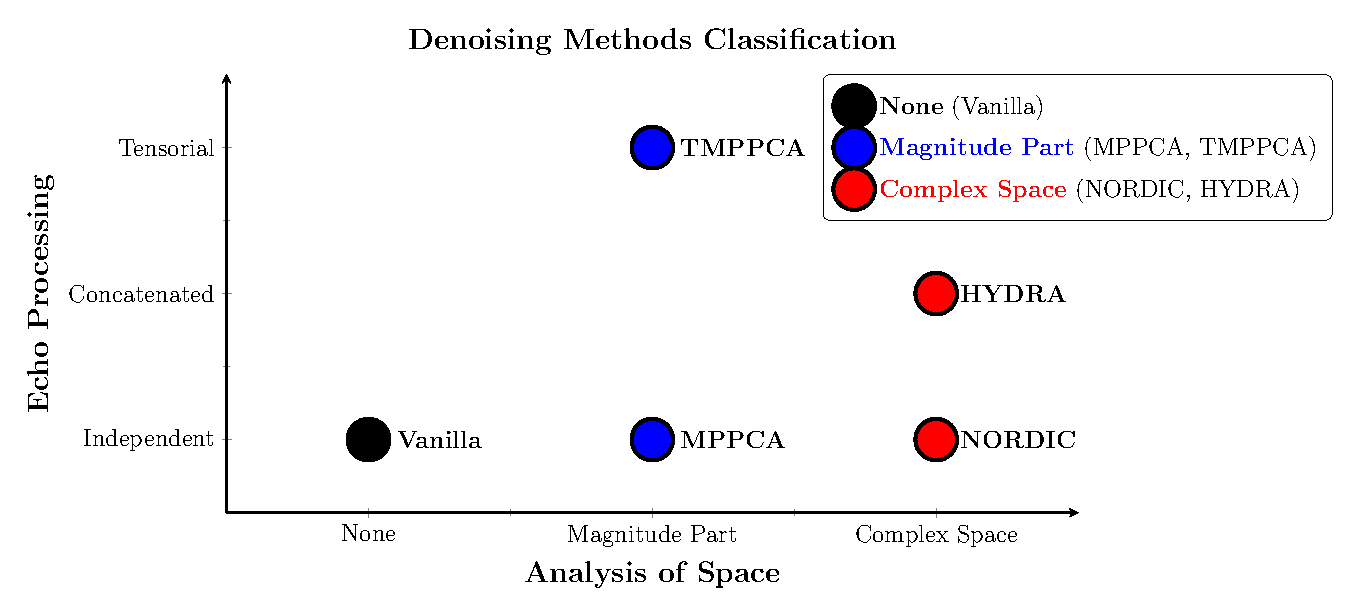
\includegraphics[width=8cm]{images/denoisingmethod.pdf}
    \caption[Characteristics of the denoising methods studied]{Characteristics of the denoising methods studied. NORDIC and HYDRA are the only methods applying thermal denoising over the complex domain, whereas TMPPCA is the only one processing all echoes at once in a tensorial form.}
    \label{fig:denoisingmethod}
\end{figure}
tMPPCA performs denoising exclusively on the magnitude component of the data, while accounting for the Rician nature of MRI noise by exploiting redundancy. However, some degree of signal leakage between tensorial dimensions has been reported, which can manifest as an apparent contrast enhancement across these dimensions. Overall, tMPPCA represents a promising and powerful alternative for denoising multi-echo data, particularly in applications where the primary objective is to maximize and exploit spatial redundancy.

\subsubsection{Aim of this thesis}
The objective of the present thesis is to investigate optimal strategies for thermal noise denoising in multi-echo data, a topic that remains insufficiently explored. Specifically, we aim to assess improvements in temporal signal-to-noise ratio (tSNR) and the accuracy of $T_2^*$ and $S_0$ estimates. In addition, we will evaluate the fidelity of the denoising process in both resting-state and task-related fMRI acquisitions. 

For resting-state data, we will quantify voxel-wise reliability using resting-state reliability analysis \citep{lynchRapidPrecisionFunctional2020}. For task-related data, we will assess the ability to predict voxel-wise activity based on a General Linear Model (GLM) fit (e.g., GLMsingle \citep{princeImprovingAccuracySingletrial2022}). This evaluation is motivated by evidence that random-matrix–based denoising methods may induce activation spreading, signal leakage between voxels, and spurious activation-like patterns \citep{fernandesMPPCADenoisingFMRI2023a, manzanopatronDenoisingDiffusionMRI2024a, kay2022risk}.



We will compare the following denoising strategies (see Fig.~\ref{fig:denoisingmethod}): (i) no denoising applied to the time series (hereafter referred to as “vanilla”), (ii) MPPCA denoising, (iii) NORDIC denoising applied independently to each echo, (iv) NORDIC applied simultaneously to all echoes by spatial concatenation (hereafter referred to as HYDRA-NORDIC), and (v) tMPPCA .

\begin{table}[H]
\centering
\caption{Thermal Denoising Methods Analysis}
\label{tab:thermal}
\small % Reduced font size
\renewcommand{\arraystretch}{1.2} % Better spacing
\begin{tabular}{@{} l c c c c @{}}
\toprule
\textbf{Method} & \textbf{Analysis Space} & \textbf{Threshold} & \textbf{Echoes} & \textbf{Extra Data} \\
\midrule
Vanilla    & -               & -            & Independent & - \\
MPPCA      & Magnitude Part  & Patch-based  & Independent & - \\
NORDIC     & Complex Space   & Whole-voxels & Independent & Phase + Noise \\
HYDRA      & Complex Space   & Whole-voxels & Concatenated & Phase + Noise \\
TMPPCA     & Magnitude Part  & Adaptive     & Tensorial    & - \\
\bottomrule
\end{tabular}
\end{table}



\end{onehalfspace}